\begin{figure}
\caption{The scene divided into three regions}
\centering
\label{fig:zones}
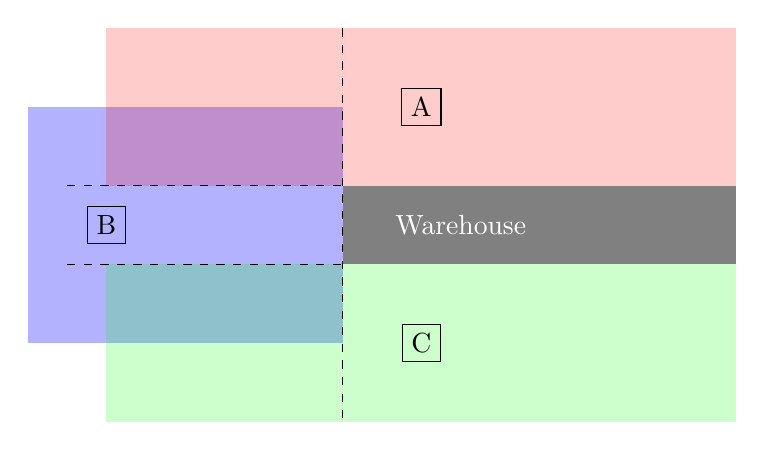
\begin{tikzpicture}  


\fill (-1,2) [fill=blue, fill opacity=0.3] rectangle (3,5);
\fill (0,4) [fill=red, fill opacity=0.2] rectangle (8,6);
\fill (0,1) [fill=green, fill opacity=0.2] rectangle (8,3);

\fill (3,3) [gray] rectangle (8,4);
\draw [dashed] (-0.5,3) -- (3,3);
\draw [dashed] (-0.5,4) -- (3,4);
\draw [dashed] (3,6) -- (3,1);

\node[draw] at (4,5) {A};
\node[draw] at (0,3.5) {B};
\node[draw] at (4,2) {C};

\node[text=white, draw=gray] at (4.5,3.5) {Warehouse};

\end{tikzpicture}
\end{figure}